% --------------------- Requirement Analysis ---------------------------------
\pagebreak

\section{Requirement Analysis}

\subsection{Requirement Matrix}
% For Requirement Matrix, latest excel should be pasted and formatted here.
\begin{figure}[H]  
    \centering
    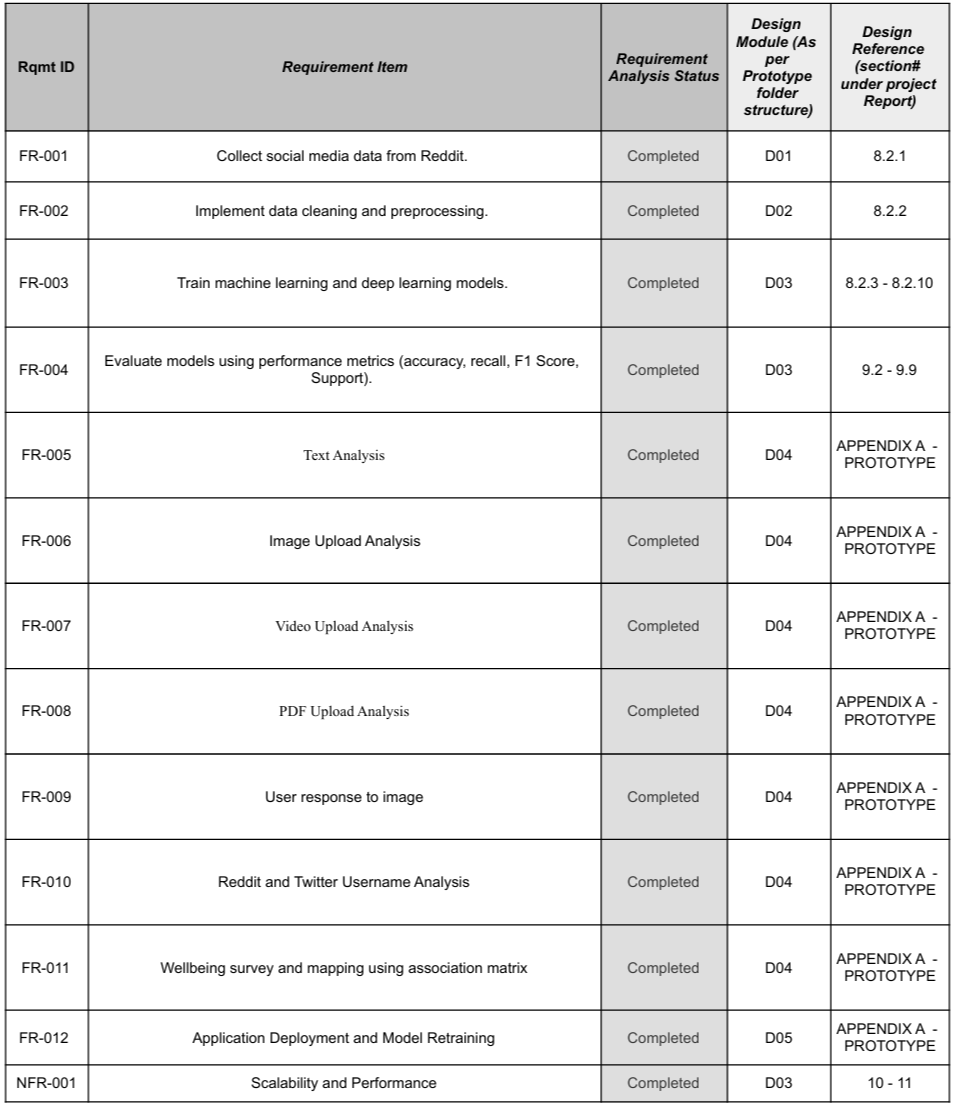
\includegraphics[width=1.0\textwidth]{Images/Requirement Matrix.png}  
    \caption*{Requirement Matrix}
    \label{Requirement Matrix}  % Label for referencing the figure
\end{figure}

\pagebreak

\subsection{Requirement Elaboration}
% Create separate sections for separate areas of requirement as in Requirement Matrix. 
% \vspace{.1in}

% \noindent
% For \textbf{Requirement Elaboration}, titles of s6.2.1, 6.2.2 etc. should be with the name of respective requirement areas. Your focus should be on: “What is needed in the system?” Requirement IDs should match with the ID column under Requirement Matrix.

\begin{table}[H]
    \centering
    \renewcommand{\arraystretch}{1.2}
    \begin{tabularx}{\textwidth}{|c|X|X|X|}
        \hline
        \textbf{No} & \textbf{Requirement} & \textbf{Input} & \textbf{Output} \\
        \hline
        FR-001 & Collect social media data from Reddit & API queries & Raw text data \\
        \hline
        FR-002 & Implement data cleaning and preprocessing & Raw text data & Cleaned, structured text \\
        \hline
        FR-003 & Train machine learning and deep learning models & Preprocessed data & Trained \newline models \\
        \hline
        FR-004 & Evaluate models using performance metrics & Trained models & Accuracy, Recall, F1 Score \\
        \hline
        FR-005 & Text Analysis & User text input & Mental disorder classification \\
        \hline
        FR-006 & Image Upload Analysis & Uploaded image & Extracted text, emotions for classification \\
        \hline
        FR-007 & Video Upload Analysis & Uploaded video & Extracted frames, emotions and text for classification \\
        \hline
        FR-008 & PDF Upload Analysis & Uploaded PDF & Extracted text and analysis \\
        \hline
        FR-009 & User response to image & User input & Mental Disorder classification based on input text \\
        \hline
        FR-010 & Reddit and Twitter \newline Username Analysis & Username input & Mental disorder trends across the top posts \\
        \hline
        FR-011 & Wellbeing survey and mapping using \newline association matrix & Survey responses & Mental health insights \\
        \hline
        FR-012 & Application \newline Deployment and Model Retraining & Updated dataset & Improved/updated model accuracy within the web application\\
        \hline
        \hline
        NFR-001 & Scalability and \newline Performance & Handling bigger dataset and subset models for a global ensemble model & Maintaining overall accuracy and response time \\
        \hline
    \end{tabularx}
    \caption*{\textbf{Functional and Non-Functional Requirements}}
\end{table}

\pagebreak
% -------------------- Requirement Analysis Ends -----------------------------
